\IEEEoverridecommandlockouts
\overrideIEEEmargins

\usepackage{cite}
\usepackage{amsmath,amssymb,amsfonts}
\usepackage{graphicx}
\usepackage{textcomp}
\usepackage{xcolor}
\usepackage{booktabs}
\usepackage{array}
\usepackage{url}
\usepackage{stfloats}

\graphicspath{{Figures/}}


\title{\LARGE \bf
Body-Motion Control of a Simulated Aerial Swarm from a First-Person View}

\author{
\authorblockN{
Yang Chen, Darius Giannoli, Dario Floreano, \textit{Fellow}, IEEE
}
\authorblockA{
Laboratory of Intelligent Systems,
EPFL, Switzerland\\
\texttt{chenyang@ai.iit.tsukuba.ac.jp},
\texttt{\{darius.giannoli,dario.floreano\}@epfl.ch}
}
\thanks{\textcolor{red}{Videos are available at
\protect\url{https://youtube.com/darius}.}}%
\thanks{This work was supported by the Swiss National Science Foundation
under Grant 200020\_212077.}%
\thanks{This study involving human participants was approved by the EPFL
Human Research Ethics Committee under Application No.\ HREC 092-2023.}%
\thanks{The authors thank Pablo Palle for his ground work on the simulation.}%
}

\begin{document}

\maketitle
\thispagestyle{empty}
\pagestyle{empty}

\begin{figure*}[b]
\centering
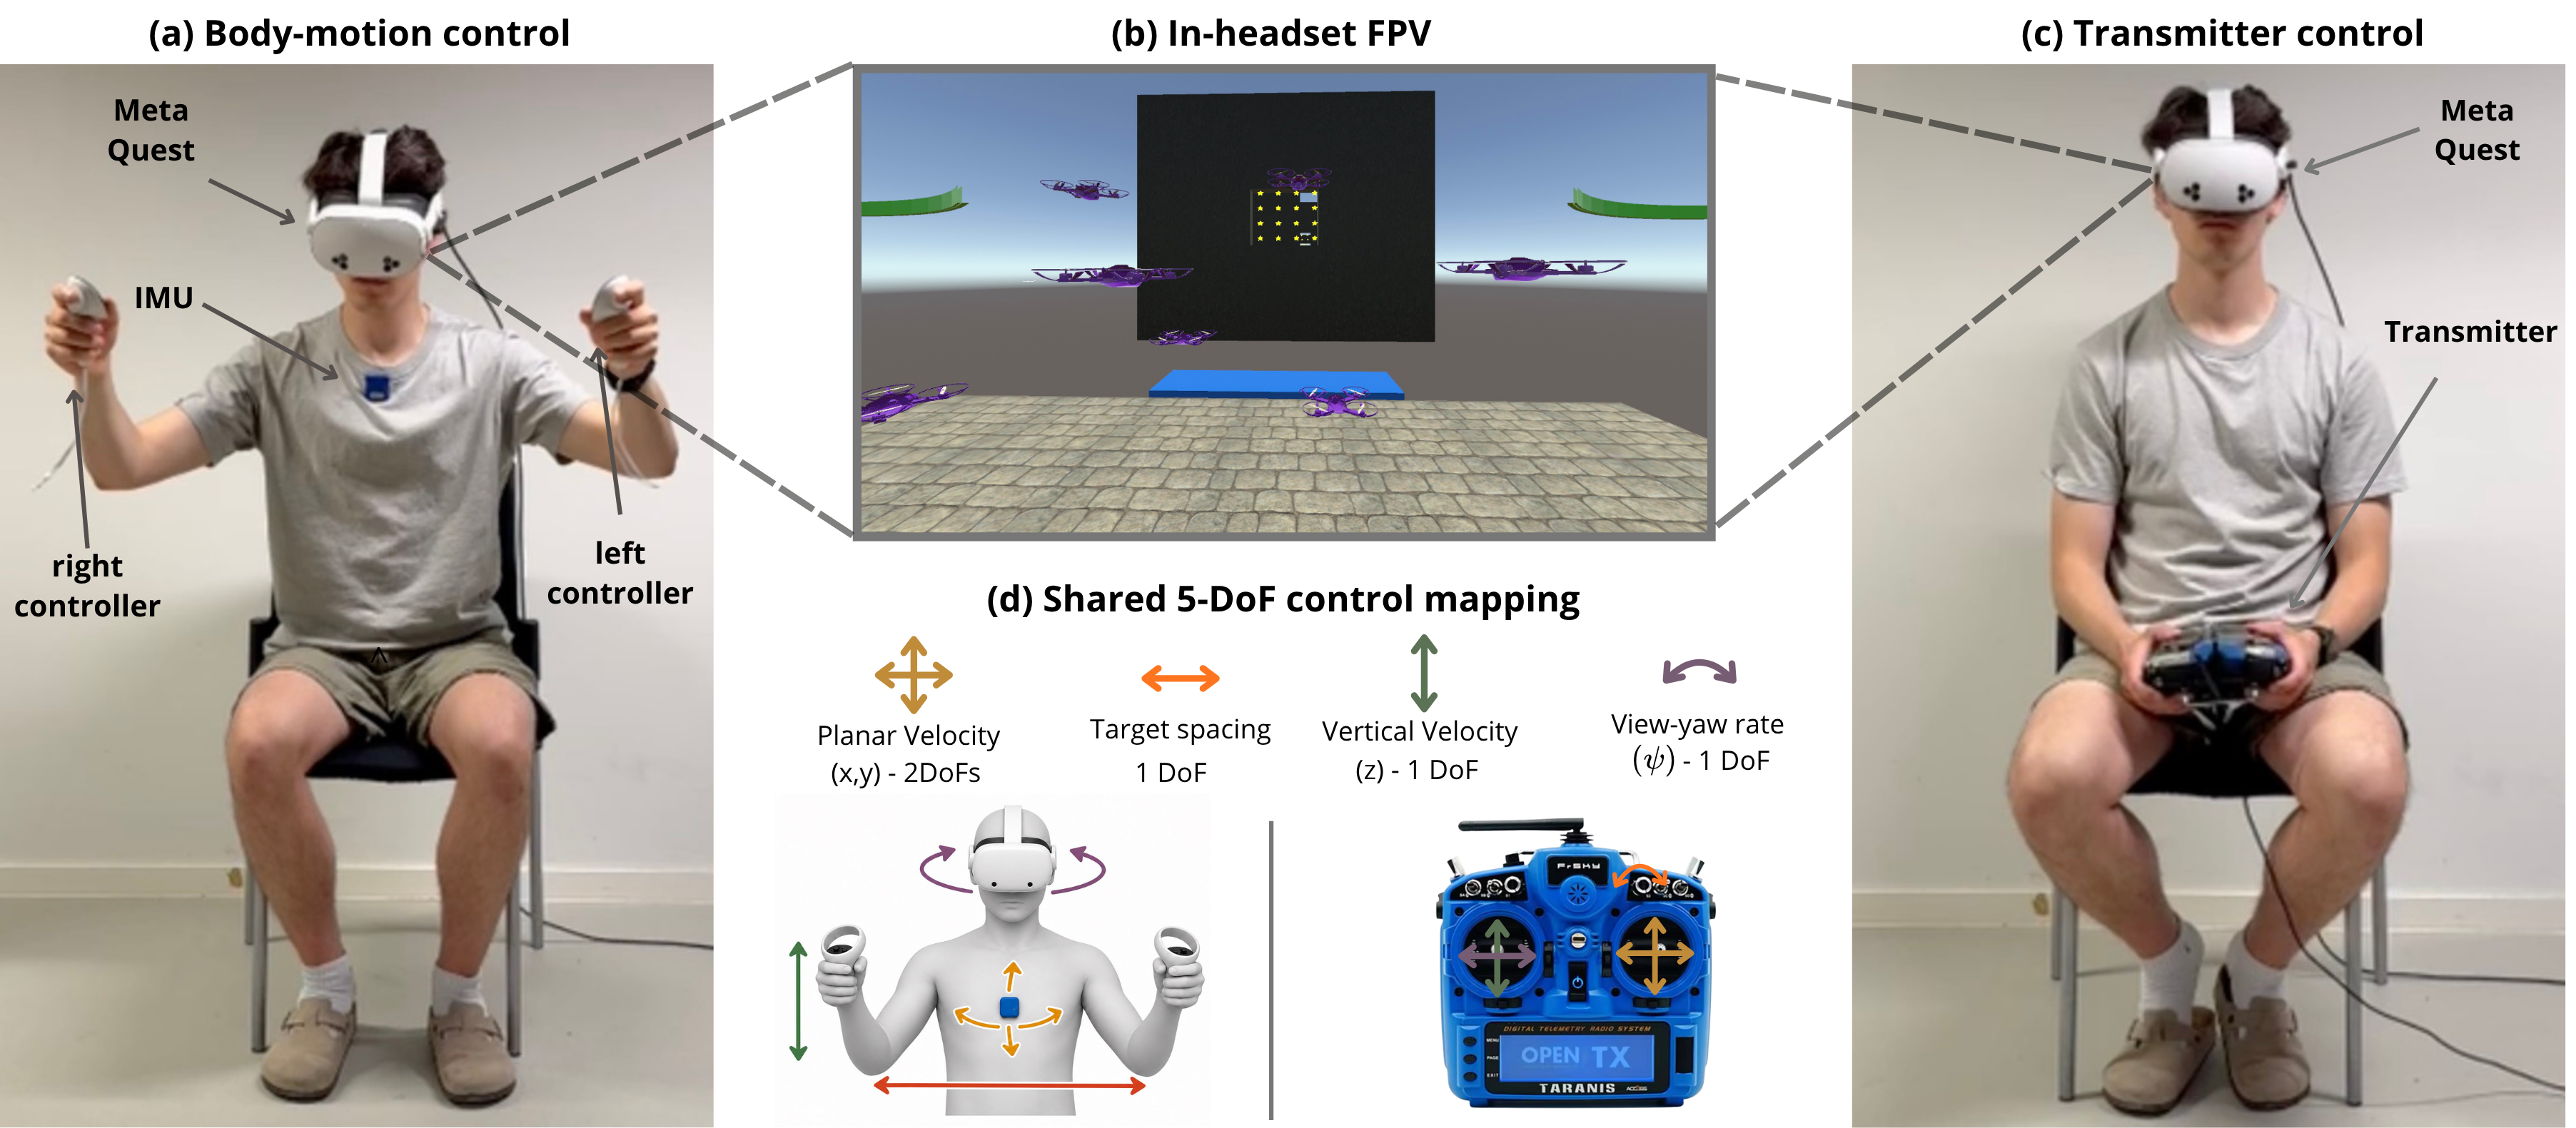
\includegraphics[width=\textwidth]{Figures/carre.png}
\caption{Overview of the within-subject experiment: (a) body-motion control,
(b) the in-headset rear-focal FPV view, (c) transmitter control, and
(d) the common five-DOF command set exposed by both interfaces: planar
velocity, vertical velocity, target spacing, and view-yaw rate.}
\label{fig:study_overview}
\end{figure*}

\begin{abstract}
Aerial-swarm teleoperation from an immersive first-person view (FPV) requires
continuous control of collective motion, view direction, and formation size.
We present a participant-calibrated upper-body interface for five-degree-of-
freedom control of a simulated aerial swarm. Torso inclination, controller
height and separation, and head yaw command planar velocity, vertical velocity,
inter-agent spacing, and view-yaw rate. In a within-subject study, 14
participants navigated a 15-agent swarm through three-dimensional obstacle
courses using body motion and a conventional transmitter. The complete
body-motion system reduced completion time by 19.4\% and centroid travel
distance by 7.0\%. An exploratory trajectory analysis also found 8.6\% less
three-dimensional cross-track motion. Delivered-command variation was lower
with body motion, although this comparison included interface-specific
filtering. No clear differences were detected in task accuracy, swarm
integrity, overall workload, or usability, whereas physical demand was higher
with body motion for all participants. These findings demonstrate a
task-specific efficiency advantage for the implemented body-motion system,
without isolating the effects of input modality, command mapping, or signal
processing.
\end{abstract}


% =====================================================================
\section{Introduction}




Aerial swarms can extend sensing and coverage by coordinating many robots, but
missions that depend on human judgment still require an interface between one
operator and the collective
\cite{kolling2016survey,ben_focaldrone}. Rather than command agents
individually, the operator can specify low-dimensional commands for collective
motion.
The present task requires five continuous command dimensions: forward and
lateral velocity, vertical velocity, view yaw rate, and formation spacing.


An external view, such as a top-down view (TDV), exposes swarm geometry, whereas a focal-agent first-person
view (FPV) can be obtained from an onboard camera without a dedicated viewing
platform. This advantage comes with restricted global awareness, a viewpoint
that moves or transfers between agents, and a command frame that rotates with
the view \cite{ben_focaldrone,macchini2021impact}. FPV yaw must therefore be
controlled together with swarm translation, altitude, and spacing.

\textit{Jarvis et al.}'s interface assigned these commands to two
transmitter sticks and a rotary control \cite{ben_focaldrone}. Although
familiar, this layout may serialize adjustments when several dimensions must
change during the same maneuver. Studies of multidimensional input distinguish
such separable operation from integral input, in which dimensions can be varied
concurrently \cite{jacob1994integrality,zhai1998quantifying}. An upper-body
interface could instead distribute commands across the head, torso, and arms
while preserving spatial correspondence between torso inclination and planar
motion in the focal agent's yaw frame.

Prior body--machine interfaces have enabled immersive or personalized control
of individual drones
\cite{rognon2018flyjacket,miehlbradt2018datadriven,macchini2024datadriven}.
At swarm level, personalized hand-motion mappings controlled four dimensions
from an external view \cite{macchini2021personalized}, while tactile and
gesture-based interfaces supported hand-guided swarm motion and aerial-formation
control \cite{tsykunov2019swarmtouch,kratky2025gesture}. Conversely,
focal-agent FPV swarm control has been studied using a conventional transmitter
\cite{ben_focaldrone}. These studies leave open whether upper-body motion can
support continuous control of swarm translation, altitude, formation spacing,
and view yaw from within the group.




We address this question with a participant-calibrated upper-body interface for
a simulated swarm. Torso inclination commands
planar velocity, mean hand height commands vertical velocity, hand separation
sets target inter-agent spacing, and head yaw commands FPV yaw rate. We compare
the complete interface with a radio-control transmitter in a within-subject
study of 14 participants navigating three-dimensional gap-passing courses. The study evaluates traversal efficiency, trajectory geometry,
delivered-command variation, task accuracy, swarm integrity, workload,
usability, and preference. Our contributions are (i) a five-dimensional body-motion mapping
aligned with the focal agent's yaw frame, including during viewpoint rotation
and transfer, and (ii) a user study showing faster and more direct traversal without
detected differences in task accuracy, swarm integrity, overall workload, or
usability, but with higher physical demand. 



% =====================================================================
\section{Swarm Control System and Input Interfaces}
% --- 2a. Methodology: the interface and the body-to-swarm mapping ---

\subsection{Shared Swarm and FPV System}
\label{sec:system}

Both input conditions generated a common five-dimensional command vector for
the simulated 15-agent swarm:
\begin{equation}
\mathbf{u}_t =
\left[
v_{\mathrm{fwd},t}^{\mathrm{ref}},
v_{\mathrm{lat},t}^{\mathrm{ref}},
v_{\mathrm{vert},t}^{\mathrm{ref}},
\dot{\psi}_{t}^{\mathrm{cmd}},
\rho_t^{*}
\right]^{\mathsf T}.
\label{eq:swarm_command}
\end{equation}
The first three components specify focal-frame horizontal and world-vertical
reference velocities, $\dot{\psi}_{t}^{\mathrm{cmd}}$ specifies FPV yaw rate,
and $\rho_t^{*}$ specifies absolute target surface-to-surface clearance.

A decentralized Olfati--Saber controller~\cite{olfatisaber2006flocking}
combined clearance regulation, velocity alignment, reference-velocity
tracking, and obstacle repulsion. At 50~Hz, an undirected interaction graph
connected agents separated by less than
$R_t=\max(2\rho_t^{*},\,\rho_t^{*}+2~\mathrm{m})$; the component containing
the focal agent defined the controlled swarm. Following Jarvis et
al.~\cite{ben_focaldrone}, the agent farthest rearward along the current
horizontal viewing direction provided the stereoscopic FPV. A handoff occurred
only when another candidate remained at least 0.5~m farther rearward for
0.5~s 

In both conditions, participants viewed the FPV through a virtual reality (VR) headset (Meta Quest 3S). For body-motion control, the headset measured head yaw, the two handheld controllers connected to the headset measured three-dimensional hand positions, and a chest-mounted inertial measurement unit (LPMS-B2 IMU) measured torso inclination. Input hardware, mapping, participant calibration, and signal processing were condition-specific; the swarm controller, command limits, focal-agent logic, and simulation were shared.

\subsection{Body-to-Swarm Mapping}
\label{sec:mapping}



At time $t$, the interface measured sagittal and lateral torso inclination
$(\theta_t,\phi_t)$, headset yaw $\psi_t$, mean controller height
\[
h_t=\frac{y^W_{L,t}+y^W_{R,t}}{2},
\]
and controller separation
\[
s_t=\left\lVert\mathbf{p}^W_{R,t}-\mathbf{p}^W_{L,t}\right\rVert .
\]
Translation and yaw were rate controlled, so a
sustained posture produced continuous motion, whereas controller separation
mapped directly to the desired formation clearance.

\emph{Participant-specific normalization:}
Each rate-controlled signal was mapped to $[-1,1]$ using its calibrated lower
extreme, neutral value, and upper extreme $(q^{-},q^{0},q^{+})$, with a
deadzone of half-width $d$ around neutral. Let
$q_{\mathrm{L}}=q^{0}-d$ and $q_{\mathrm{U}}=q^{0}+d$. The normalization was
\begin{equation}
\mathcal{D}(q_t;q^{-},q^{0},q^{+},d)=
\begin{cases}
\displaystyle
\max\!\left(-1,
\frac{q_t-q_{\mathrm{L}}}{q_{\mathrm{L}}-q^{-}}\right),
& q_t<q_{\mathrm{L}},\\[6pt]
0,
& q_{\mathrm{L}}\leq q_t\leq q_{\mathrm{U}},\\[3pt]
\displaystyle
\min\!\left(1,
\frac{q_t-q_{\mathrm{U}}}{q^{+}-q_{\mathrm{U}}}\right),
& q_t>q_{\mathrm{U}}.
\end{cases}
\label{eq:deadzone_mapping}
\end{equation}
Separate scaling on either side of neutral accommodated asymmetric ranges of
motion.


\begin{figure}[!t]
\centering
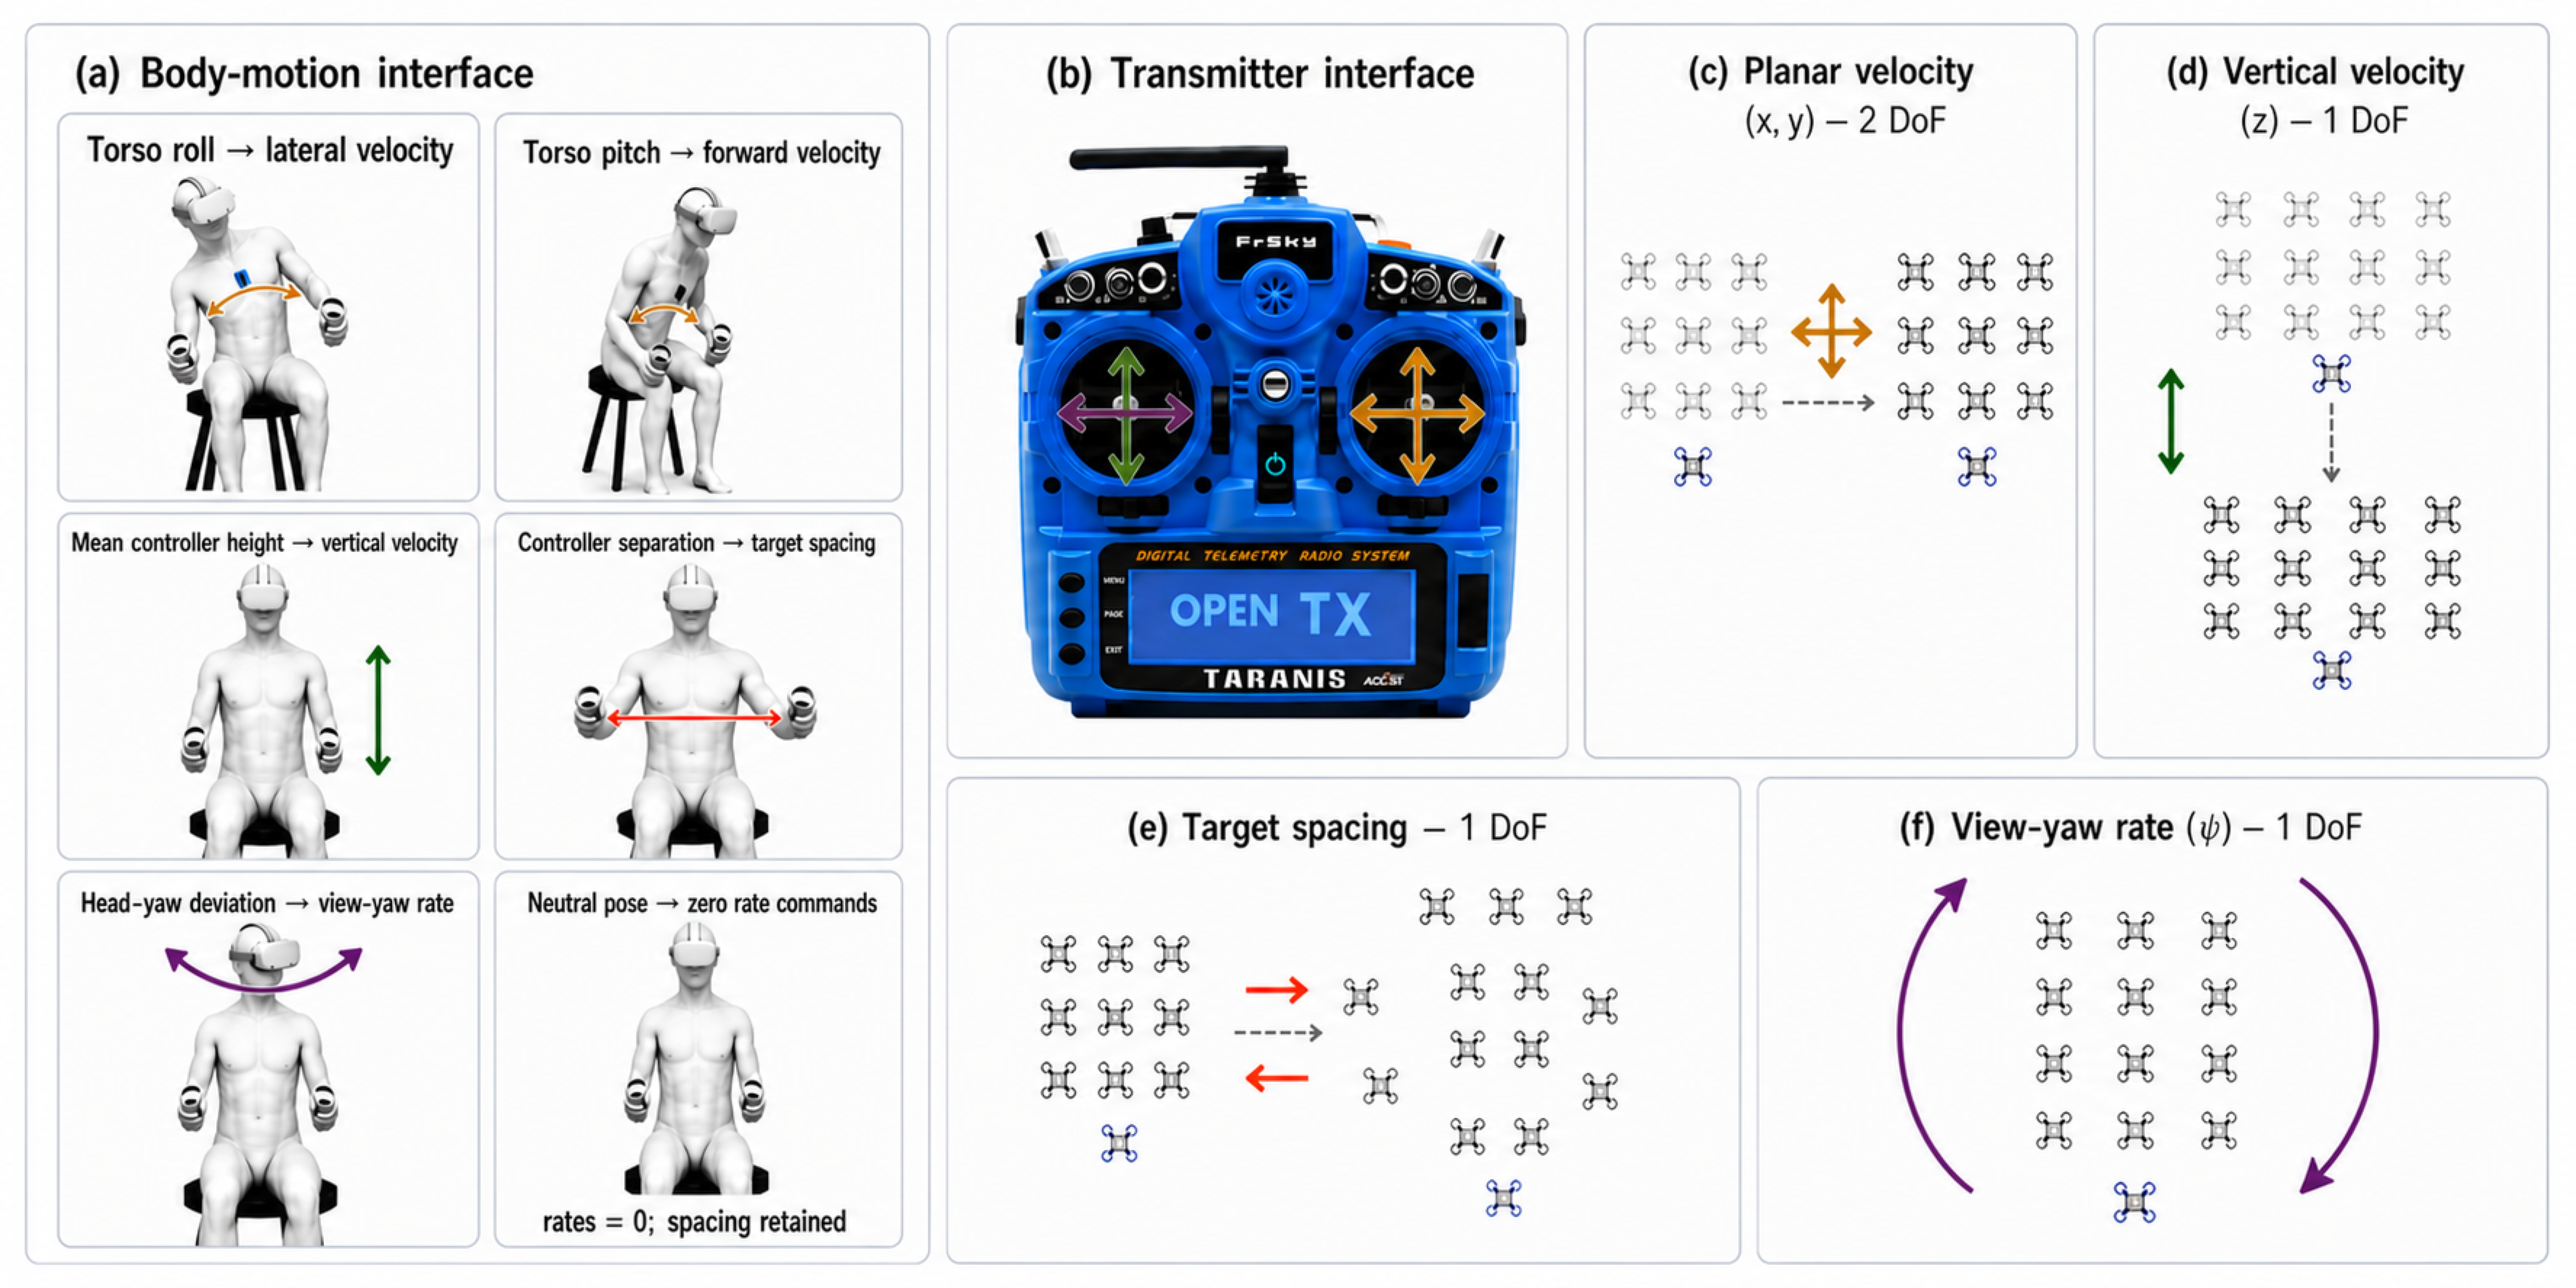
\includegraphics[width=\linewidth]{Figures/hom.png}
\caption{Body-to-swarm control mappings: (a) torso roll controls lateral
velocity, (b) torso pitch controls forward velocity, (c) mean controller
height controls vertical velocity, (d) controller separation controls target
spacing, and (e) head-yaw deviation controls view-yaw rate. (f) The neutral
pose produces zero rate commands while retaining the current target-spacing
setpoint. Faded formations illustrate the direction of the commanded swarm
motion, scaling, or view rotation.}
\label{fig:mapping}
\end{figure}


\emph{Translation:}
The normalized translation commands were
\begin{align}
c_{\mathrm{fwd},t}
&=\mathcal{D}(\theta_t;\theta^{-},0,\theta^{+},5^{\circ}),
\nonumber\\
c_{\mathrm{lat},t}
&=\mathcal{D}(\phi_t;\phi^{-},0,\phi^{+},5^{\circ}),
\nonumber\\
c_{\mathrm{vert},t}
&=\mathcal{D}(h_t;h_{\min},h_0,h_{\max},0.05~\mathrm{m}).
\label{eq:body_rate_commands}
\end{align}
Positive commands denoted forward, rightward, and upward motion. The normalized
commands were smoothed, with the resulting values denoted by
$(\bar c_{\mathrm{fwd},t},\bar c_{\mathrm{lat},t},
\bar c_{\mathrm{vert},t})$. These values were then scaled by
$10~\mathrm{m\,s^{-1}}$ to obtain the corresponding reference velocities
$(v_{\mathrm{fwd},t}^{\mathrm{ref}},v_{\mathrm{lat},t}^{\mathrm{ref}},
v_{\mathrm{vert},t}^{\mathrm{ref}})$ in Eq.~\eqref{eq:swarm_command}.
The forward and lateral velocities were defined relative to the displayed
heading and updated after FPV rotation or viewpoint transfer.

\emph{Inter-agent spacing:}
Controller separation $s_t$ was linearly mapped from the participant-specific
range $[s_{\min},s_{\max}]$ to a target surface-to-surface clearance
$\rho_t\in[1,5]~\mathrm{m}$. The mapping was clipped at the calibrated limits and
smoothed to produce the applied command $\rho_t^*$ in
Eq.~\eqref{eq:swarm_command}. Because this was an absolute mapping,
participants selected the desired clearance directly rather than commanding
an expansion or contraction rate.

\emph{FPV yaw:}
With
$\Delta\psi_t=
\operatorname{wrap}_{[-180^{\circ},180^{\circ})}
(\psi_t-\psi_{0,t})$
denoting the head-yaw deviation from its neutral orientation, the FPV yaw-rate
command was
\begin{equation}
\dot{\psi}^{\,\mathrm{cmd}}_t
=
48^{\circ}\mathrm{s}^{-1}
\mathcal{D}\!\left(
\Delta\psi_t;\psi_{\mathrm{L}},0,\psi_{\mathrm{R}},10^{\circ}
\right).
\label{eq:yaw_rate}
\end{equation}
Returning the head to neutral stopped FPV rotation without restoring the
previous viewing direction. The neutral yaw was slowly adapted during periods
of head stillness to compensate for postural drift. No additional yaw
smoothing was applied.

The fixed gains, deadzones, and smoothing settings were selected through pilot
and informal testing.

\subsection{Participant-Specific Calibration}
\label{sec:calibration}

Each participant completed a one-time guided 13-pose calibration to record
seated neutral postures and comfortable motion limits. The chair configuration and Quest tracking origin remained fixed thereafter.

Calibration included five torso poses (neutral and maximum forward, backward,
left, and right), three head-yaw poses (neutral and maximum left and right),
two controller-separation poses (minimum and maximum), and three
controller-height poses (minimum, neutral, and maximum). Neutral torso and head
poses defined the IMU orientation offset and headset yaw reference $\psi_0$,
respectively; only $(s_{\min},s_{\max})$ parameterized the absolute spacing
mapping.

The measured bounds directly parameterized the translation, yaw-rate, and
spacing mappings.
Table~\ref{tab:calibration_summary} summarizes the resulting spans; angular
spans combine opposing excursions, whereas position spans are
maximum--minimum differences.

\begin{table}[!tb]
\centering
\caption{Calibrated input spans across participants ($N=14$).}
\label{tab:calibration_summary}
\footnotesize
\setlength{\tabcolsep}{3.5pt}
\begin{tabular}{@{}lcc@{}}
\toprule
Input span & Mean $\pm$ SD & Range \\
\midrule
Sagittal torso ($^\circ$)       & $56.4 \pm 18.4$  & $34.2$--$98.1$ \\
Lateral torso ($^\circ$)        & $52.0 \pm 18.0$  & $26.2$--$81.2$ \\
Head yaw ($^\circ$)             & $117.5 \pm 24.7$ & $65.6$--$138.0$ \\
Controller separation (m)       & $1.10 \pm 0.33$  & $0.70$--$1.51$ \\
Controller height (m)           & $0.77 \pm 0.22$  & $0.43$--$1.22$ \\
\bottomrule
\end{tabular}
\end{table}

\subsection{Transmitter Baseline}
\label{sec:transmitter}

A conventional radio-control transmitter (FrSky Taranis X9D Plus) generated the same command vector, $\mathbf{u}_t$, as the body-motion interface. The right stick controlled planar
velocity, the left horizontal axis controlled FPV yaw rate, the
non-self-centering left throttle controlled vertical velocity, and the right
rotary knob set target inter-agent clearance. Stick axes used a symmetric 0.12
deadzone with rescaling of the remaining range, while the knob mapped linearly
to $\rho^*\in[1,5]$~m. Both conditions used the same command limits and
yaw-aligned reference frame. The transmitter received no participant-specific
calibration or additional temporal filtering.

% =====================================================================

\label{sec:experiment}

\section{Experimental Evaluation}
\label{sec:experiment}


\subsection{Participants and Study Design}
\label{sec:participants_design}

The study included $N=14$ adults recruited from the local university
community (10 men and 4 women; age: $22.4 \pm 4.0$ years, range 19--35).
Sample size reflected participant availability; no a priori power analysis was
conducted. Eligibility required self-reported ability to perform the seated
upper-body movements and vision compatible with the VR headset. All
participants completed the study, provided written informed consent, and were
compensated.

A two-condition within-subject design compared the body-motion and transmitter
interfaces described in Sections~\ref{sec:system}--\ref{sec:transmitter}. The
first participant's starting interface was selected at random and alternated
thereafter, yielding seven participants per sequence. Both conditions were
completed while seated during a single session lasting approximately 1~h.




\subsection{Task and Procedure}
\label{sec:task}

\begin{figure}[t]
\centering
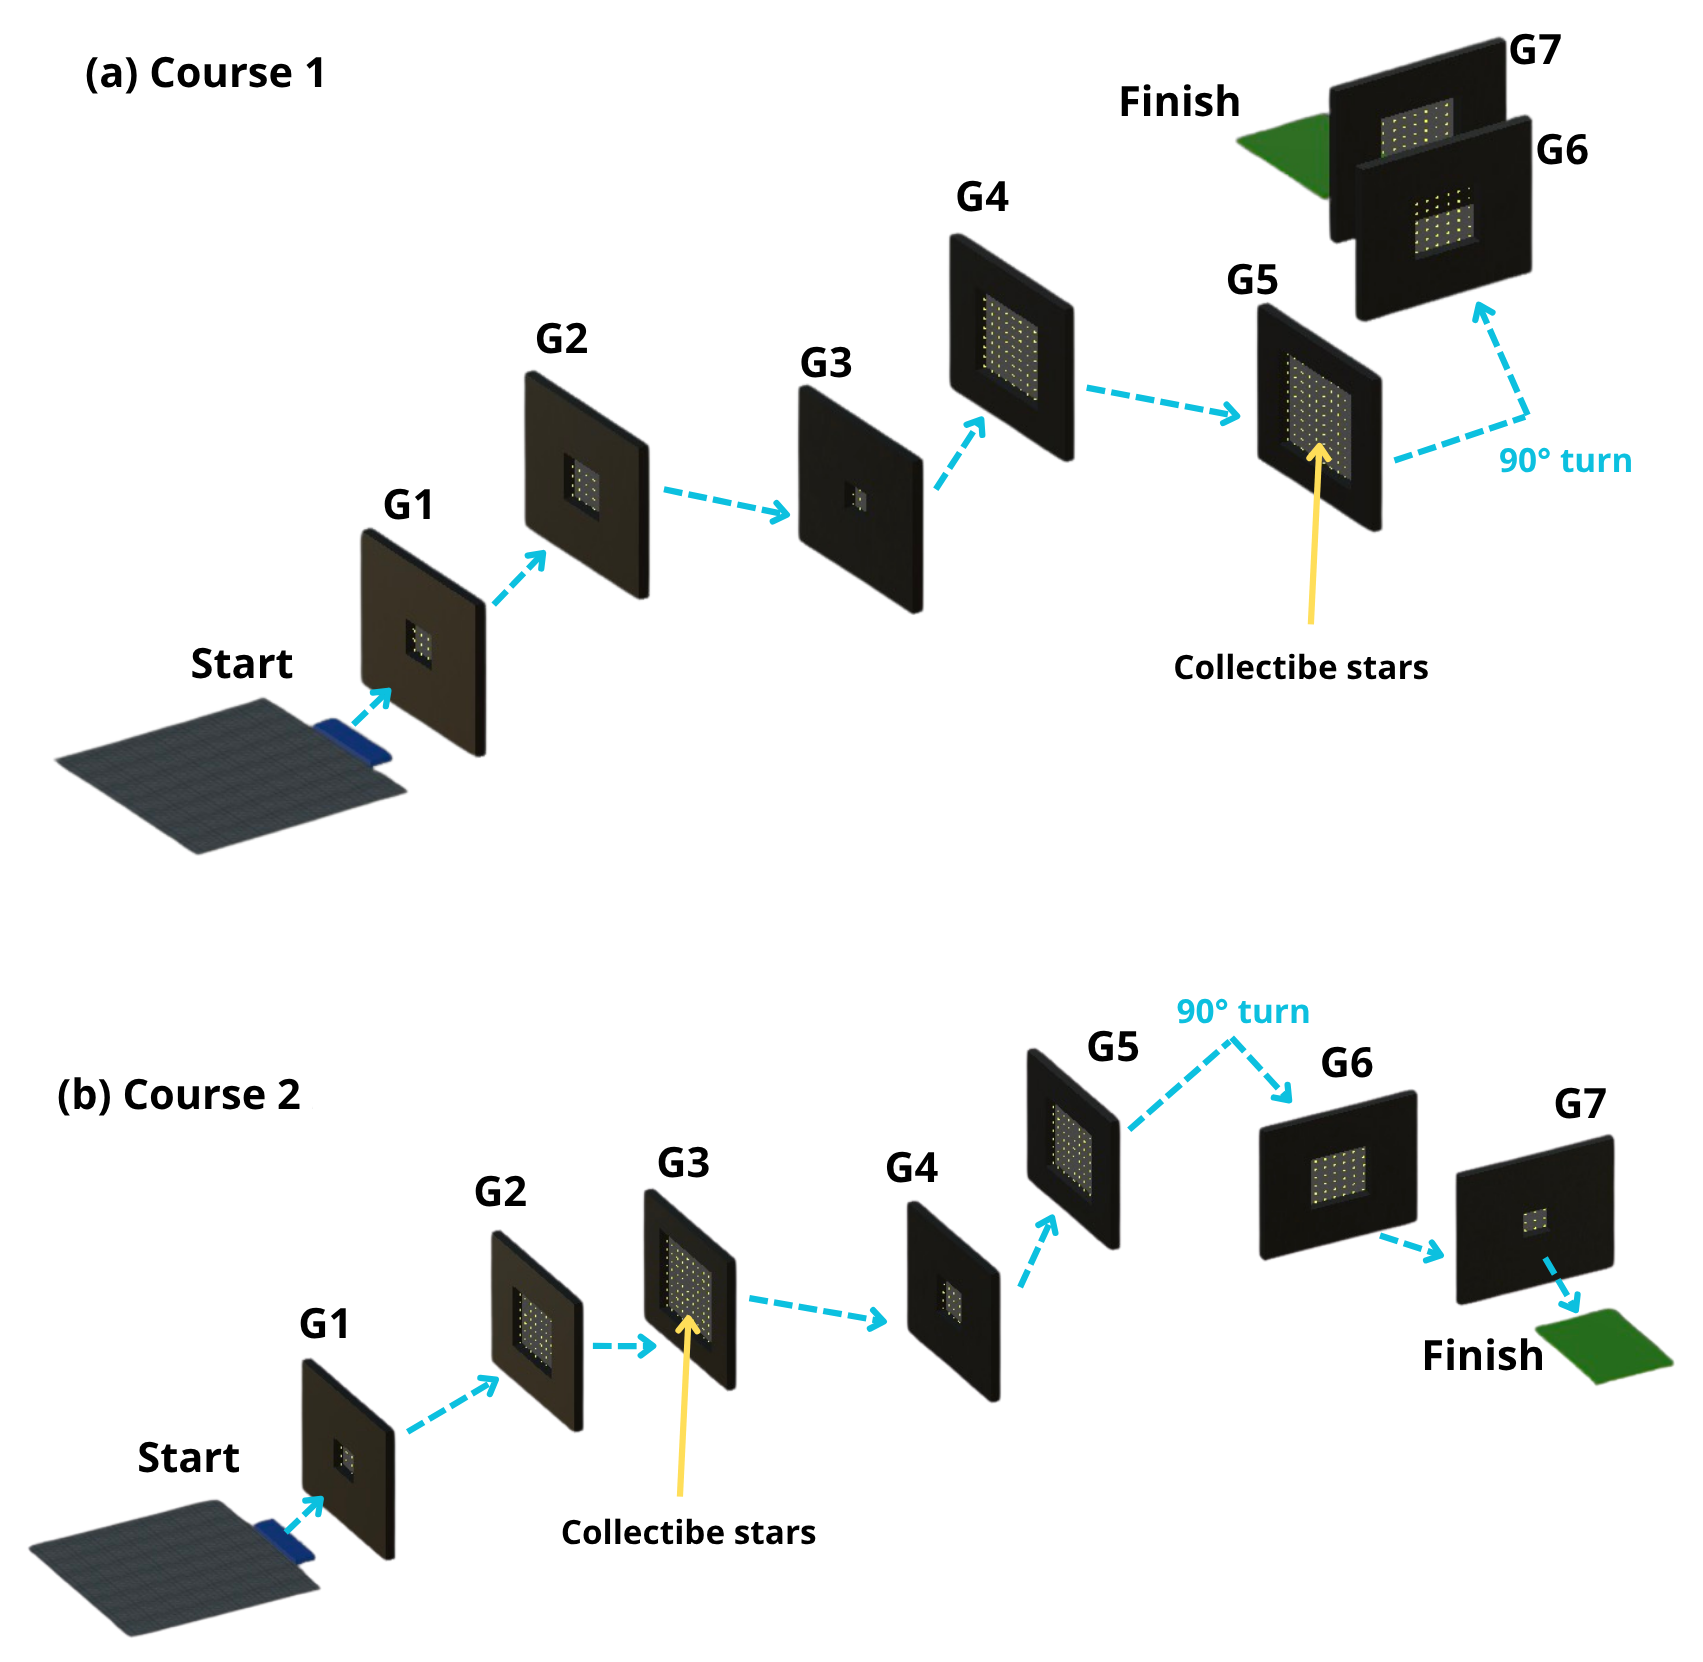
\includegraphics[width=\columnwidth]{Figures/layouts.png}
\caption{Recorded-course layouts for (a) trial~1 and (b) trial~2.
Labels G1--G7 mark the gate sequence; dashed arrows show traversal direction.}
\label{fig:course_layouts}
\end{figure}


All participants received identical prerecorded instructions and
demonstrations. They were asked to complete each course as quickly as possible while passing near the opening centers, collecting stars, and minimizing crashes and disconnections. Control remained active during the approach, providing a flying start. Timing ran from the first agent crossing the start plane to the first agent crossing the finish plane. A run was valid only if the controlled-component centroid crossed all seven gate planes in sequence; no time limit was imposed. Participants viewed only stereoscopic FPV, with no timer, score, or task-status display.

A star was collected when any agent entered its trigger; wall or inter-agent collisions removed the affected agent, and survivors outside the interaction graph's largest connected component were classified as disconnected at each sample.

Before the body-motion block, participants completed the calibration described
in Section~\ref{sec:calibration}. Each interface block began with familiarization
on the practice course: participants first maneuvered freely with standardized
experimenter guidance and then completed one unrecorded full-course traversal.
Two recorded runs followed in fixed order.

After each interface block, participants completed the weighted NASA Task Load
Index (NASA-TLX)~\cite{hart1988nasatlx} and the 10-item System Usability Scale
(SUS)~\cite{brooke1996sus}, referring only to the two recorded runs. After both
blocks, they reported interface preference and relative motion sickness
(body motion, transmitter, or no difference) and could provide optional
free-text comments.

\subsection{Outcome Measures}

We evaluated the interfaces in terms of \textbf{traversal efficiency}, \textbf{movement
characteristics}, \textbf{delivered-command behavior}, \textbf{task performance and swarm
integrity}, and \textbf{subjective experience}.

\emph{Traversal efficiency.}
Completion time $T$ was measured between the recorded start and finish events
and served as the primary performance outcome. Centroid path length $L$ was the
cumulative three-dimensional distance travelled by the controlled component,
and mean speed was computed as $\bar v=L/T$. Lower completion time and path
length, and higher mean speed, indicated more efficient traversal.

\emph{Movement characteristics.}
Movement continuity was characterized by the time spent below $0.5~\mathrm{m\,s^{-1}}$
and the number of low-speed episodes lasting at least $0.5$~s. Segment
straightness was defined as the summed endpoint-to-endpoint distance of the
eight course segments divided by the corresponding centroid path length.
We further measured the fraction of incremental motion orthogonal to the direct
three-dimensional segment directions, $C_{\perp}$, and excess vertical travel,
$V_{\mathrm{exc}}$. Lower low-speed time, episode count, $C_{\perp}$, and
$V_{\mathrm{exc}}$, and higher straightness, indicated more continuous and
direct movement.

To characterize path directness, we performed a post-hoc gate-to-gate
decomposition. For each of the eight start--gate, gate--gate, and gate--finish
segments, $\hat{\mathbf{u}}_j$ denotes the unit vector along its endpoint chord.
We computed
\begin{equation}
\begin{aligned}
C_{\perp}
&=
\frac{
\sum_j\sum_k
\left\|
\Delta\mathbf{x}_{j,k}
-(\Delta\mathbf{x}_{j,k}^{\mathsf T}\hat{\mathbf{u}}_j)
 \hat{\mathbf{u}}_j
\right\|_2
}{
\sum_j\sum_k\lVert\Delta\mathbf{x}_{j,k}\rVert_2
},\\
V_{\mathrm{exc}}
&=
\sum_j
\left(
\sum_k |\Delta y_{j,k}|
-
|y_{j,K_j}-y_{j,1}|
\right).
\end{aligned}
\label{eq:trajectory_geometry}
\end{equation}
Lower $C_{\perp}$ indicates that a larger fraction of movement followed the
direct three-dimensional segment directions. Lower $V_{\mathrm{exc}}$
indicates less vertical reversal beyond the endpoint-to-endpoint height change.
We also examined the vertical component of gate-centering error separately.

\emph{Delivered-command behavior.}
The five delivered commands---three translations, target spacing, and
view-yaw rate---were normalized by their implemented ranges to
$\mathbf{q}_k\in[0,1]^5$. With $\tau=t_M-t_1$,
$\Delta\mathbf{q}_k=\mathbf{q}_{k+1}-\mathbf{q}_k$, and
$\Delta t_k=t_{k+1}-t_k$, delivered-command variation was
\begin{equation}
E_{\mathrm{cmd}}=
\frac{\tau}{5}
\sum_{k=1}^{M-1}
\frac{\lVert\Delta\mathbf{q}_k\rVert_2^2}{\Delta t_k}.
\label{eq:command_metrics}
\end{equation}
Lower values indicate less variation in the commands supplied to the swarm,
not necessarily better performance. Because the interfaces used different
online filters, this metric characterizes the complete delivered-command
pipelines rather than intrinsic input smoothness.


\emph{Task accuracy and swarm integrity.}
At the first ordered forward crossing of each gate, normalized gate-centering
error was
\begin{equation}
E_{\mathrm{gate}}=\frac{1}{7}\sum_{g=1}^{7}
\max\left(\frac{|h_g|}{W_g/2},\frac{|v_g|}{H_g/2}\right),
\label{eq:gate_error}
\end{equation}
where $h_g,v_g$ are offsets from the opening center and $W_g,H_g$ are its
dimensions. Values of zero and one indicate the opening center and edge,
respectively. We further measured unique-star collection yield, swarm survival
($1-N_{\mathrm{crash}}/15$), and the time-weighted fraction of surviving
agents in the largest connected component.

\emph{Subjective measures.}
NASA-TLX and SUS quantified workload and usability. Weighted TLX, its six
0--100 dimension ratings, and Raw TLX were analyzed. Interface preference and
relative motion sickness were summarized descriptively.

\subsection{Data Processing and Statistical Analysis}
\label{sec:statistical_analysis}

All 56 runs were retained. Seven participants began with body motion and seven
with the transmitter. Metrics were computed from the native 15-Hz samples
without additional smoothing or resampling. The two courses were averaged
within participant and interface, yielding 14 paired observations.

Interfaces were compared using exact two-sided Wilcoxon signed-rank tests
($\alpha=.05$). Holm correction was applied separately within the traversal,
task-outcome, primary-subjective, and TLX-dimension families. The post-hoc
trajectory family comprised $C_{\perp}$, $V_{\mathrm{exc}}$, and vertical
gate-centering error; the single delivered-command outcome required no
adjustment. Body-minus-transmitter mean differences are reported with
paired-bootstrap 95\% confidence intervals based on 20,000 resamples.
Sensitivity checks examined course, condition order, path sampling, common
additional filtering, and Raw TLX scoring.

% =====================================================================
\section{Results}

Paired analyses included all 14 participants and are presented below.

\begin{figure}[!tb]
\centering
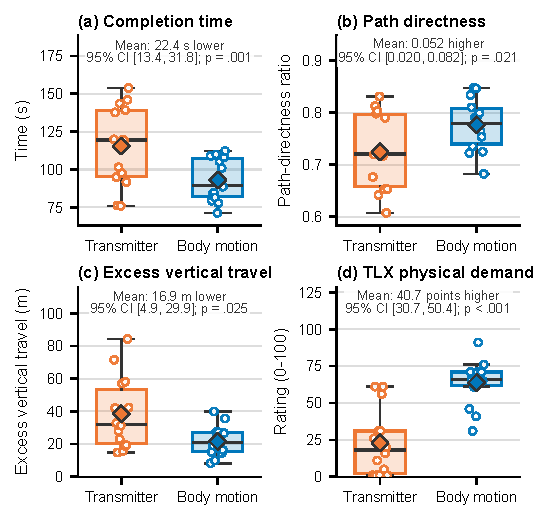
\includegraphics[width=\columnwidth]{Figures/fig_paired_results_2x2.pdf}
\caption{Paired outcomes: (a) completion time, (b) 3-D cross-track
fraction, (c) excess vertical travel, and (d) TLX physical demand. Lines
connect interfaces, open symbols denote participants, and diamonds denote
means. Annotations report body-minus-transmitter differences, bootstrap 95\%
CIs, and Holm-adjusted $p_{\mathrm H}$ values. Panels (b,c) are post hoc.}
\label{fig:paired_results}
\end{figure}

\emph{Traversal efficiency.}
Body motion reduced completion time from 115.4 to 93.0~s, a 19.4\% reduction
($\Delta=-22.4$~s; 95\% CI $[-31.8,-13.4]$;
$p_{\mathrm H}=.001$); 13 of 14 participants were faster
(Fig.~\ref{fig:paired_results}(a)). Paths were 7.0\% shorter
(298.6 versus 321.1~m; $p_{\mathrm H}=.011$), and mean speed was 12.5\%
higher (3.27 versus 2.91~m/s; $p_{\mathrm H}=.001$).

Post hoc decomposition indicated more continuous and direct motion. Time below
0.5~m/s decreased from 13.23 to 2.45~s ($\Delta=-10.78$~s; 95\% CI
$[-14.30,-7.42]$; $p_{\mathrm H}<.001$), and sustained low-speed episodes
decreased from 6.68 to 1.39 per trial ($p_{\mathrm H}<.001$).
Gate-to-gate straightness increased from 0.725 to 0.776
($\Delta=0.052$; 95\% CI $[0.021,0.082]$;
$p_{\mathrm H}=.011$).

\emph{Trajectory geometry.}
The 3-D cross-track fraction decreased by 8.6\%, from 0.552 to 0.505
($\Delta=-0.047$; 95\% CI $[-0.070,-0.023]$;
$p_{\mathrm H}=.007$), with lower values for 12 of 14 participants
(Fig.~\ref{fig:paired_results}(b)). Excess vertical travel decreased by
44.0\%, from 38.5 to 21.6~m ($\Delta=-16.9$~m; 95\% CI
$[-30.1,-4.9]$; $p_{\mathrm H}=.049$;
Fig.~\ref{fig:paired_results}(c)). Figure~\ref{fig:trajectory_overlays}
shows the corresponding horizontal paths and height profiles.

\begin{figure*}[!t]
\vspace{-2mm}
\centering
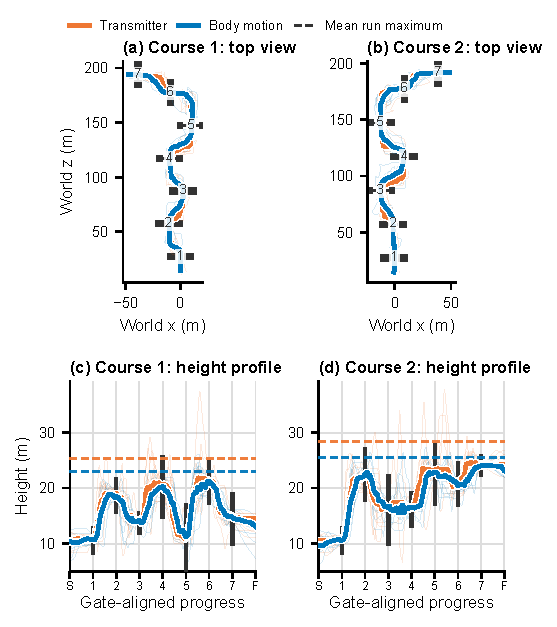
\includegraphics[width=\linewidth]
{Figures/fig_trajectory_overlays_height_mean_max.pdf}
\vspace{-1mm}
\caption{Centroid trajectories for both courses. Panels (a,b) show top views,
and panels (c,d) show gate-aligned height profiles. Thin curves are individual
runs, thick curves are interface medians, and dashed lines indicate the mean
run-wise maximum height.}
\label{fig:trajectory_overlays}
\vspace{-2mm}
\end{figure*}

\emph{Delivered-command behavior.}
Delivered-command variation was 88.8\% lower in the implemented body-motion
pipeline ($p_{\mathrm H}<.001$). Applying the same additional 0.143-s
low-pass filter to both delivered streams preserved an approximately 80.0\%
reduction. Because pre-filter body commands were not logged, this comparison
characterizes the complete pipelines rather than input modality alone.

\emph{Task outcomes.}
No clear interface difference was detected in gate centering, collection,
survival, or largest-component retention. Survival and connectivity remained
near ceiling with both interfaces; these results do not establish equivalent
task performance or safety.

\emph{Subjective outcomes.}
Weighted TLX showed no clear interface difference ($\Delta=7.2$; 95\% CI
$[-5.5,20.2]$), nor did SUS. Physical demand, however, increased from 23.0
to 63.7 and was higher with body motion for all participants
($\Delta=40.7$; 95\% CI $[30.7,50.4]$;
$p_{\mathrm H}<.001$; Fig.~\ref{fig:paired_results}(d)). Eight participants
preferred body motion, five preferred the transmitter, and one reported no
preference. Motion-sickness reports were mixed.

\FloatBarrier

% =====================================================================
\section{Discussion}

Body motion enabled faster and more direct traversal: participants completed
the courses 19.4\% faster, followed shorter paths, spent less time moving
slowly, and showed lower cross-track motion. Excess vertical travel was also
lower, although this post hoc effect was close to the significance threshold.
These related measures indicate that the advantage arose through more
continuous and direct movement, but they are not independent confirmations of
the completion-time result.

Both interfaces exposed the same five continuous DOF; body motion changed
their physical allocation rather than their number. Delivered commands were less variable with body motion. However, the interfaces
differed in hardware, calibration, mapping, and filtering. The results therefore compare
the implemented end-to-end systems and do not isolate the effects of body input,
DOF allocation, or signal processing.

The efficiency advantage was not accompanied by a detected difference in gate
centering, collection, survival, or connectivity. This provides no evidence of
a measured task-performance trade-off, but ceiling effects and the small sample
prevent claims of equivalence or comparable safety. Body motion also imposed a
clear physical cost, despite no detected difference in total TLX or SUS.
Arm support or smaller-excursion gains may reduce effort
\cite{rognon2018flyjacket}, while formation-clearance feedback could improve
spatial awareness \cite{tsykunov2019swarmtouch}.

These findings extend upper-body control from individual aerial robots and
externally viewed formations
\cite{rognon2018flyjacket,miehlbradt2018datadriven,
macchini2024datadriven,macchini2021personalized}
to rear-focal FPV swarm teleoperation.

Future work should use larger samples, counterbalanced courses,
longer exposure, and harder tasks; record commands before and after processing;
and match or ablate interface mappings and filtering. Physical-swarm studies
are needed to test whether the efficiency advantage persists under
communication, aerodynamic, and safety constraints.

% \begin{figure}[t]
% \centering
% \includegraphics[width=\columnwidth]{Figures/fig_traj_comparison.png}
% \caption{LOL TRAJ LOL}
% \label{fig:paired_results}
% \end{figure}
% =====================================================================
\section{Conclusion}


We presented a participant-calibrated upper-body interface for continuous five-DOF FPV swarm teleoperation. In a 14-participant within-subject study, the complete body-motion system reduced completion time by 19.4\% relative to a
transmitter, with 7.0\% shorter paths, higher mean speed, and lower
delivered-command variation. However, physical demand increased, while no differences were detected in task accuracy, swarm integrity, total workload, or usability; these null results do not establish equivalence. Matched-processing and physical-swarm studies are needed to isolate modality effects and determine whether the efficiency advantage generalizes beyond the tested simulated 15-agent rear-FPV task.


% =====================================================================
\bibliographystyle{IEEEtran}
\bibliography{references}

\end{document}
